\documentclass{article}
\usepackage[utf8]{inputenc}

\usepackage{graphicx}
\usepackage{natbib}

\title{IF669 - Introdução a Programação}
\author{Maria Clara Alencastro Braner Kenderessy}
\date{Dezembro, 2021}

\begin{document}

\maketitle

\begin{figure}[h]
    \centering
    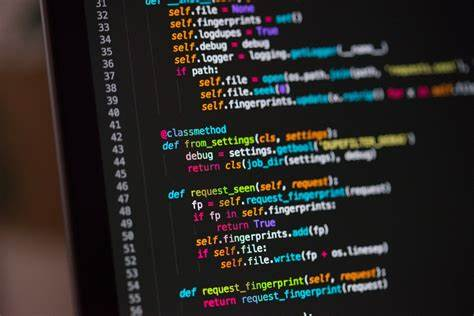
\includegraphics[scale=0.6]{projetoic_img.jpg}
    \caption{Código escrito em Python}
    \label{fig:mesh1}
\end{figure}

\section{Introdução}

\hspace{0.5in}A disciplina de introdução a programação é uma cadeira obrigatória oferecida no primeiro período dos cursos de Ciência da Computação e Engenharia da Computação. Possui uma carga horária total de 120 horas e é ministrada pelos professores Filipe Calegario, Ricardo Massa e Sérgio Soares.

\paragraph{\hspace{0.5in}A disciplina tem como ementa conceitos básicos de linguagens de programação e de programação orientada a objetos e qualidade de software, estruturas de controle e estrutura de dados composta, ambiente de programação, conceitos básicos de programação imperativa, padrões e arquitetura de software, além de estilos de programação e projeto de implementação.}

\section{Relevância}

\hspace{0.5in}Introdução a programação tem uma metodologia de ensino focada em trazer conceitos básicos da programação, os quais são imprescindíveis para o aprendizado de outras linguagens. 

\paragraph{\hspace {0,5in}Ademais, é voltada para fortalecer o desenvolvimento lógico computacional do aluno, buscando o aprendizado por trás da programação, assim como entender formas de fazer certas funções que já são inseridas no contexto da programação.}

\section{Relação com outras disciplinas}

No curso de Ciência da Computação na UFPE a cadeira de Introdução a Programação funciona como pré-requisito para as seguintes disciplinas:

\begin{itemize}
  \item IF672 - Algoritmos e estrutura de dados.
  \item IF674 - Infra-estrutura de Hardware
  \item IF677 - Infra-estrutura de Software
  \item IF678 - Infra-estrutura de comunicação
  \item IF681 - Interfaces usuário-máquina
  \item IF683 - Projeto de desenvolvimento
  \item IF687 - Introdução a multimídia
\end{itemize}

\cite{livro1}
\cite{site}
\cite{livro2}

\bibliographystyle{plain}
\bibliography{ref}

\end{document}
